\documentclass{beamer}
\usepackage{pifont}
\mode<presentation>
{
\usetheme{default}      % or try Darmstadt, Madrid, Warsaw, ...
\usecolortheme{default} % or try albatross, beaver, crane, ...
\usefonttheme{default}  % or try serif, structurebold, ...
\setbeamertemplate{navigation symbols}{}
\setbeamertemplate{caption}[numbered]
}

\usecolortheme[named=black]{structure}
\usepackage[english]{babel}
\usepackage[utf8x]{inputenc}

\setbeamercolor{footcolor}{fg=gray,bg=white}%
\setbeamertemplate{footline}{%
  \leavevmode%
  \hbox{%
   \begin{beamercolorbox}[wd=1\paperwidth,ht=2.3ex,dp=2.3ex,right]{footcolor}%
    Survey and Literature Review \hspace*{1cm} {\scriptsize\insertframenumber{}/\inserttotalframenumber}\hspace*{3ex}
   \end{beamercolorbox}}%
  \vskip0pt%
}

\usepackage[english]{babel}
\usepackage[utf8x]{inputenc}
\usepackage{tikz}
\usetikzlibrary{shapes,arrows}


\renewcommand\mathfamilydefault{\rmdefault}
\renewcommand{\math}[1]{\ensuremath{\boldsymbol{#1}}} % bold math
\newcommand{\R}{\mathbb{R}}
\newcommand{\norm}[1]{|#1|}

% TikZ styles for drawing
\usetikzlibrary{arrows,shapes,shadows,positioning,automata,patterns}
\usetikzlibrary{trees,decorations.pathmorphing,decorations.markings}
\usetikzlibrary{shapes.geometric,backgrounds,calc}


% TikZ styles for drawing
\tikzstyle{block} = [draw,rectangle,rounded corners,thick,minimum height=2em,minimum width=2cm,fill=gray!20,draw=black!50]
\tikzstyle{sum} = [draw,circle,inner sep=0mm,minimum size=5mm,thick,fill=white!40,draw=black!50]



%% Title =================================================================
\title{Survey and Literature Review on Distributed Observers}
\subtitle{\small Spring 2020}
\author{NAME}
\institute{@njust.edu.cn}
\date{\scriptsize\color{gray} Spring 2020}





\begin{document}

%%--------------------------------------------------------
\begin{frame}
\titlepage
\thispagestyle{empty}
\end{frame}
%%--------------------------------------------------------



%%--------------------------------------------------------
\begin{frame}
\thispagestyle{empty}

\setbeamertemplate{section in toc}[sections numbered]
\tableofcontents%[hideallsubsections]

\end{frame}
%%--------------------------------------------------------





%%========================================================
\section{Review of Paper: TAC-62(2)-2017}%

%%--------------------------------------------------------
\begin{frame}
\thispagestyle{empty}

\begin{center}
{\large\bf\color{blue}Paper: TAC-62(2)-2017 \\
{\small ``Design of Distributed LTI Observers for State Omniscience''} \\
{\small By S.~Park and N.~C.~Martins}}
\end{center}
\end{frame}
%%--------------------------------------------------------



\subsection{\ding{228}~Centralized vs distributed observers}%

%%--------------------------------------------------------
\begin{frame}{\color{blue} Centralized vs distributed observers}

Consider LTI plant in state-space form
\begin{equation*}
x^{+}=A x,~~ x\in\R^{n}
\end{equation*}

\begin{itemize}
  \item Centralized observer:
\begin{equation*}
y=Cx \in\R^{r}
\end{equation*}
is available to ensure $(C,A)$ is observable or detectable

  \item Distributed observer:
\begin{equation*}
y_{i}=C_{i}x\in\R^{r_{i}},~~ r_{i}\geq0,~~ i=1,2,\cdots,m
\end{equation*}
the system can be accessed \textbf{separately} at $m$ places, though
\begin{equation*}
(C,A) ~~\text{with}~~ C=\begin{bmatrix} C_{1} \\ \vdots \\ C_{m} \\   \end{bmatrix}\in\R^{r} ~~\text{is observable}
\end{equation*}
\end{itemize}

\end{frame}
%%--------------------------------------------------------




%%--------------------------------------------------------
\begin{frame}{\color{blue} }

\begin{columns}[onlytextwidth]
\column{0.5\textwidth}
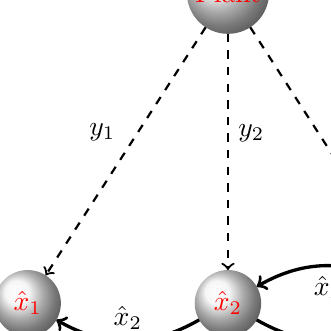
\begin{tikzpicture}[node distance=1.7cm]
\useasboundingbox (0,0) rectangle (3.5,3.5);
  \tikzset{VertexStyle/.style = {shape          = circle,
                                 ball color     = gray!10,
                                 text           = red,
                                 inner sep      = 2pt,
                                 outer sep      = 0pt,
                                 minimum size   = 24 pt}}

     \node[VertexStyle](A){ \math{\hat{x}_{1}} };
     \node[VertexStyle,right=of A](B){\math{\hat{x}_{2}}};
     \node[VertexStyle,right=of B](C){\math{\hat{x}_{3}}};
     \node[VertexStyle,above=3cm of B](P){Plant};

     \draw[thick,->,dashed](P) to node[above right]{ \math{y_{2}} } (B);
     \draw[thick,->,dashed](P) to node[above left]{ \math{y_{1}} } (A);
     \draw[thick,->,dashed](P) to node[above right]{ \math{y_{3}} } (C);

     \draw[very thick,->,bend left](B) to node[above]{\math{\hat{x}_{2}}} (A);
     \draw[very thick,->,bend right](B) to node[below]{\math{\hat{x}_{2}}} (C);
     \draw[very thick,->,bend right](C) to node[below]{\math{\hat{x}_{3}}} (B);
\end{tikzpicture}

\column{0.45\textwidth}
Plant with $m$ outputs
\begin{align*}
x^{+}&=A x \\
y_{i}&=C_{i}x,~~ i=1,\cdots, m
\end{align*}
Distributed observer:
\begin{align*}
\hat{x}^{+}_{i}&=f_{i}(\hat{x}_{i},y_{i},\hat{x}_{j},j\in\mathcal{N}_{i})  \\
\mathcal{N}_{i}&~\text{``neighbors''} \\
& i=1,\cdots, m
\end{align*}
\end{columns}

\vskip 0.5cm

Centralized (Luenberger) observer:
\begin{align*}
\hat{x}^{+} &= A \hat{x} + L(y-C\hat{x}),~~ C=\begin{bmatrix} C_{1} \\ \vdots \\ C_{m} \\   \end{bmatrix}
\end{align*}

NOT realistic! Paper: TAC-62(2)-2017 is a result in this direction

\end{frame}
%%--------------------------------------------------------





\subsection{\ding{228}~Problem description}%
%%--------------------------------------------------------
\begin{frame}{\color{blue} Notation}

\begin{itemize}
  \item The number of observers is a fixed integer
\begin{equation*}
m\geq 1
\end{equation*}

  \item A graph formed by a vertex set $\mathbb{V}$ and an edge set $\mathbb{E}$ is denoted by
\begin{equation*}
\mathcal{G}=(\mathbb{V},\mathbb{E}) ~~\text{with}~~ \mathbb{E}\subseteq\mathbb{V}\times\mathbb{V}
\end{equation*}

  \item $\otimes$ is the Kronecker product

  \item $\text{diag}(K_{1},\cdots,K_{p})$ is the block diagonal matrix

  \item

  \item

  \item
\end{itemize}


\end{frame}
%%--------------------------------------------------------




%%--------------------------------------------------------
\begin{frame}{\color{blue} Plant and its outputs}
Consider LTI plant in state-state form
\begin{equation*}
x^{+}=A x,~~ y=Cx,~~ x\in\R^{n},~~ y\in\R^{r}
\end{equation*}
with
\begin{equation*}
y=\begin{bmatrix} y_{1} \\ \vdots \\ y_{m} \\   \end{bmatrix},~~ C=\begin{bmatrix} C_{1} \\ \vdots \\ C_{m} \\   \end{bmatrix},~~
y_{i}=C_{i}x\in\R^{r_{i}},~~ i=1,\cdots,m
\end{equation*}
\end{frame}
%%--------------------------------------------------------




%%--------------------------------------------------------
\begin{frame}{\color{blue} The distributed observer by Park-Martins}

Structure of the observers
\begin{align*}
\hat{x}^{+}_{i}&=A\sum_{j\in\mathbb{N}_{i}} {\bf w}_{ij}\hat{x}_{j} + {\bf K}_{i}(y_{i}-C_{i}\hat{x}_{i})+ {\bf P}_{i}z_{i} \\
z^{+}_{i}&={\bf Q}_{i}(y_{i}-C_{i}\hat{x}_{i})+ {\bf S}_{i}z_{i},~~ i=1,\cdots,m
\end{align*}
where the \textbf{augmented state}
\begin{equation*}
z_{i}\in\R^{\mu_{i}},~~ \sum_{i=1}^{m}\mu_{i}<m
\end{equation*}
The latter is referred to as the \textbf{scalability condition}

\end{frame}
%%--------------------------------------------------------




%%--------------------------------------------------------
\begin{frame}{\color{blue} }
\begin{itemize}
  \item Input and output of the $i$th observer
\begin{center}
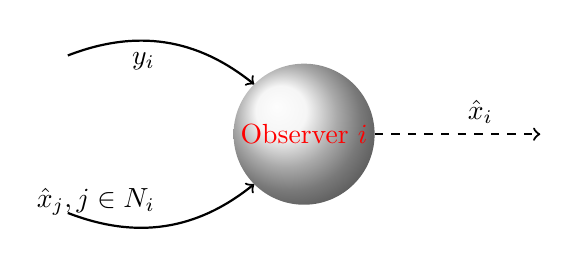
\begin{tikzpicture}[node distance=1.7cm]
  \tikzset{VertexStyle/.style = {shape          = circle,
                                 ball color     = gray!10,
                                 text           = red,
                                 inner sep      = 2pt,
                                 outer sep      = 0pt,
                                 minimum size   = 24 pt}}

     \node[VertexStyle](A){ Observer \math{i}  };

     \draw[thick,->,bend left](-3,1) to node[below left]{ \math{y_{i}} } (A.north west);
     \draw[thick,->,bend right](-3,-1) to node[above left]{ \math{\hat{x}_{j},j\in\mathbb{N}_{i}} } (A.south west);

     \draw[thick,->,dashed](A) to node[above right]{ \math{\hat{x}_{i}} } (3,0);
\end{tikzpicture}
\end{center}

\begin{align*}
\hat{x}^{+}_{i}&=A\sum_{j\in\mathbb{N}_{i}} {\bf w}_{ij}\hat{x}_{j} + {\bf K}_{i}(y_{i}-C_{i}\hat{x}_{i})+ {\bf P}_{i}z_{i} \\
z^{+}_{i}&={\bf Q}_{i}(y_{i}-C_{i}\hat{x}_{i})+ {\bf S}_{i}z_{i},~~ i=1,\cdots,m
\end{align*}


  \item It is hoped
\begin{equation*}
\lim_{k\rightarrow\infty} |\hat{x}_{i}(k)-x(k)|=0  ~~\text{and}~~ \sum_{i=1}^{m}\mu_{i}<m-m_{s}
\end{equation*}
where $m_{s}\geq0$ is the number of \textbf{source components}
\end{itemize}

\end{frame}
%%--------------------------------------------------------





%%========================================================
\section{Review of Paper: Wang-Morse TAC-63(7)-2018}%

%%--------------------------------------------------------
\begin{frame}
\thispagestyle{empty}

\begin{center}
{\large\bf\color{blue}Paper: Wang-Morse TAC-63(7)-2018 \\
{\small ``A Distributed Observer for a Time-Invariant Linear System''} \\
{\small By L.~Wang and A.~S.~Morse}}
\end{center}
\end{frame}
%%--------------------------------------------------------



\subsection{\ding{228}~Introduction}%

%%--------------------------------------------------------
\begin{frame}{\color{blue} Plant and graph}

Consider LTI plant in state-space form
\begin{align*}
\dot{x}(t)&=A x(t) \\
y_{i}(t)&=C_{i}x(t),~~ x\in\R^{n},~~ y_{i}\in\R^{s_{i}},~~ i\in{\bf m}\triangleq \{1,2,\cdots,m\}
\end{align*}
Suppose that
\begin{equation*}
(C,A) ~~\text{with}~~ C=\begin{bmatrix} C_{1} \\ \vdots \\ C_{m} \\   \end{bmatrix}\in\R^{r} ~~\text{is observable}
\end{equation*}
For each $i\in{\bf m}$,
\begin{center}
$\mathcal{N}_{i}$ is the neighbors (with self-loops) of the $i$th observer
\end{center}
\end{frame}
%%--------------------------------------------------------






%%--------------------------------------------------------
\begin{frame}{\color{blue} Illustration}

\begin{center}
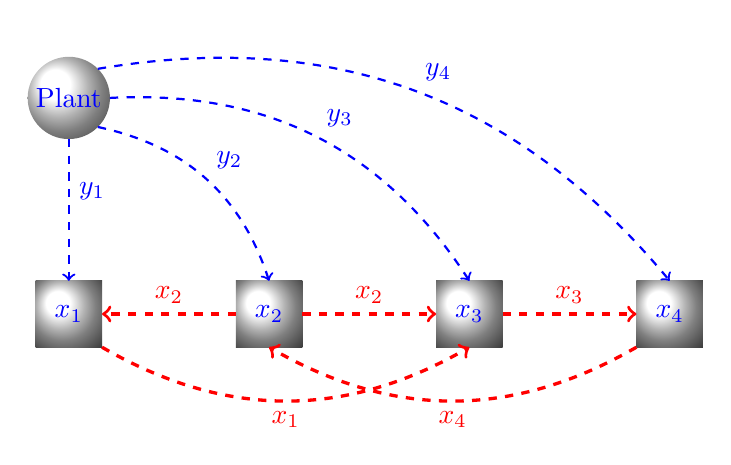
\begin{tikzpicture}[node distance=1.7cm]
  \tikzset{VertexStyle/.style = {shape          = circle,
                                 ball color     = white!20,
                                 text           = blue,
                                 inner sep      = 2pt,
                                 outer sep      = 0pt,
                                 minimum size   = 24 pt}}

     \node[VertexStyle,rectangle](A){ \math{x_{1}} };
     \node[VertexStyle,rectangle,right=of A](B){\math{x_{2}}};
     \node[VertexStyle,rectangle,right=of B](C){\math{x_{3}}};
     \node[VertexStyle,rectangle,right=of C](D){\math{x_{4}}};
     \node[VertexStyle,above=1.8cm of A](P){Plant};

     \draw[thick,->,dashed,blue](P.south) to node[above right]{ \math{y_{1}} } (A.north);
     \draw[thick,->,dashed,blue,bend left](P.south east) to node[above right]{ \math{y_{2}} } (B.north);
     \draw[thick,->,dashed,blue,bend left](P.east) to node[above right]{ \math{y_{3}} } (C.north);
     \draw[thick,->,dashed,blue,bend left](P.north east) to node[above right]{ \math{y_{4}} } (D.north);

     \draw[very thick,->,dashed,red](B.west) to node[above]{\math{x_{2}}} (A.east);
     \draw[very thick,->,dashed,red](B.east) to node[above]{\math{x_{2}}} (C.west);
     \draw[very thick,->,dashed,red](C.east) to node[above]{\math{x_{3}}} (D.west);

     \draw[very thick,->,dashed,bend right,red](A.south east) to node[below]{\math{x_{1}}} (C.south);
     \draw[very thick,->,dashed,bend left,red](D.south west) to node[below]{\math{x_{4}}} (B.south);
\end{tikzpicture}
\end{center}

\begin{align*}
m&=4,~~ {\bf m}\triangleq \{1,2,3,4\} \\
\mathcal{N}_{1}&=\{1,2\},~~ \mathcal{N}_{2}=\{2,4\},~~ \mathcal{N}_{3}=\{1,2,3\},~~ \mathcal{N}_{4}=\{3,4\}
\end{align*}

\end{frame}
%%--------------------------------------------------------





%%--------------------------------------------------------
\begin{frame}{\color{blue} Distributed observer by Wang-Morse}

Structure of the distributed observer by Wang-Morse
\begin{align*}
\dot{z}_{i}(t)&=\sum_{j\in\mathcal{N}_{i}} \Big( H_{ij}z_{j}(t) + K_{ij}y_{j}(t) \Big) \\
x_{i}(t)&=\sum_{j\in\mathcal{N}_{i}} \Big( M_{ij}z_{j}(t) + N_{ij}y_{j}(t) \Big),~~ i\in{\bf m}
\end{align*}
It achieves convergence of the estimation error
\begin{equation*}
\lim_{t\rightarrow\infty} |\epsilon_{i}(t)|=0,~~ \epsilon_{i}(t)=x_{i}(t)-x(t),~~ \forall i\in{\bf m}
\end{equation*}
\end{frame}
%%--------------------------------------------------------


%%--------------------------------------------------------
\begin{frame}{\color{blue} }

In what follows, instead of the above, we focus on a class of distributed observers of the form
\begin{align*}
\dot{z}_{i}(t)&=\sum_{j\in\mathcal{N}_{i}} H_{ij}z_{j}(t) + K_{i}y_{i}(t),~~ i\in{\bf m}
\end{align*}
with outputs
\begin{equation*}
x_{i}(t)=\sum_{j\in\mathcal{N}_{i}} M_{ij}z_{j}(t),~~ i\in{\bf m}
\end{equation*}
as the estimates of the trajectory $x(t)\in\R^{n}$ of the plant

\end{frame}
%%--------------------------------------------------------




%%--------------------------------------------------------
\begin{frame}{\color{blue} }

For the distributed observers of the form
\begin{align*}
\dot{z}_{i}(t)&=\sum_{j\in\mathcal{N}_{i}} H_{ij}z_{j}(t) + K_{i}y_{i}(t),~~ x_{i}(t)=\sum_{j\in\mathcal{N}_{i}} M_{ij}z_{j}(t),~~ i\in{\bf m}
\end{align*}
it should ensure convergence of the estimation error
\begin{equation*}
\lim_{t\rightarrow\infty} |\epsilon_{i}(t)|=0,~~ \epsilon_{i}(t)=x_{i}(t)-x(t),~~ \forall i\in{\bf m}
\end{equation*}


\begin{itemize}
  \item \textbf{Assumption} (Wang-Morse 2018TAC) The composite system is \emph{jointly observable}, i.e.
\begin{equation*}
(C,A) ~~\text{with}~~ C=\begin{bmatrix} C_{1} \\ \vdots \\ C_{m} \\   \end{bmatrix}\in\R^{r} ~~\text{is observable},~~ C_{i}\neq0,~~ \forall i\in{\bf m}
\end{equation*}


  \item \textbf{Design parameters}
\begin{equation*}
i\in{\bf m} ~:~ \big\{(H_{ij}, K_{i}, M_{ij}) : j\in\mathcal{N}_{i}\big\}
\end{equation*}
\end{itemize}
\end{frame}
%%--------------------------------------------------------





%%--------------------------------------------------------
\begin{frame}{\color{blue} }

Wang-Morse observer
\begin{align*}
\dot{z}_{i}(t)&=\sum_{j\in\mathcal{N}_{i}} H_{ij}z_{j}(t) + K_{i}y_{i}(t),~~ x_{i}(t)=\sum_{j\in\mathcal{N}_{i}} M_{ij}z_{j}(t),~~ i\in{\bf m}
\end{align*}

\begin{itemize}

  \item \textbf{Comparison} with Park-Martins observer:

\begin{itemize}
  \item First, we outline a construction for
systems with \textbf{strongly connected neighbor graphs} that enables
one to freely adjust the observer’s spectrum.

  \item Second, the results \textbf{apply whether $A$ is singular or not}; the implication
of this generalization is that the construction proposed
can be used to craft observers for continuous time processes,
whereas the construction proposed in [Park-Martins 2017TAC] cannot unless $A$ is nonsingular.
\end{itemize}
\end{itemize}
\end{frame}
%%--------------------------------------------------------




\subsection{\ding{228}~Observer design equations}%

%%--------------------------------------------------------
\begin{frame}{\color{blue} Observer design equations}

Consider the plant
\begin{equation*}
\Sigma_{plant}:~~ \dot{x}=A x,~~ y_{i}=C_{i}x,~~ i\in{\bf m}
\end{equation*}
and its observer
\begin{align*}
\Sigma_{obs}:~~ \dot{z}_{i}&=\sum_{j\in\mathcal{N}_{i}} H_{ij}z_{j} + K_{i}y_{i},~~ x_{i}=\sum_{j\in\mathcal{N}_{i}} M_{ij}z_{j},~~ i\in{\bf m}
\end{align*}

\begin{itemize}
  \item \textbf{Invariance property}\footnote{Recall the so-called \textbf{regulator equations} or \textbf{internal model property}} There should exist \textbf{``immersions''}
\begin{center}
{\color{red}from $x$ system to each $z_{i}$ system, written by $\theta_{i}(x)$ }
\end{center}
such that
\begin{align*}
\frac{\partial\theta_{i}(x)}{\partial x}Ax&=\sum_{j\in\mathcal{N}_{i}} H_{ij}\theta_{j}(x) + K_{i}C_{i}x \\
x&=\sum_{j\in\mathcal{N}_{i}} M_{ij}\theta_{j}(x),~~ i\in{\bf m},~~ \forall x\in\R^{n}
\end{align*}
\end{itemize}
\end{frame}
%%--------------------------------------------------------




%%--------------------------------------------------------
\begin{frame}{\color{blue} }

\begin{itemize}
  \item \textbf{Invariance property} There are \textbf{``immersions''} {\color{red} $\theta_{i}(x)\in\R^{n}$ } such that
\begin{align*}
\frac{\partial\theta_{i}(x)}{\partial x}Ax&=\sum_{j\in\mathcal{N}_{i}} H_{ij}\theta_{j}(x) + K_{i}C_{i}x \\
x&=\sum_{j\in\mathcal{N}_{i}} M_{ij}\theta_{j}(x),~~ i\in{\bf m},~~ \forall x\in\R^{n}
\end{align*}

  \item [] Or equivalently, there are {\color{red} linear mappings $\theta_{i}(x)=V_{i}x$} for $i\in{\bf m}$ such that
\begin{align*}
V_{i}A&=\sum_{j\in\mathcal{N}_{i}} H_{ij}V_{j} + K_{i}C_{i},~~
I_{n}=\sum_{j\in\mathcal{N}_{i}} M_{ij}V_{j},~~ i\in{\bf m}
\end{align*}
namely \textbf{``observer design equations''} in the paper
\end{itemize}
\end{frame}
%%--------------------------------------------------------







\subsection{\ding{228}~Solvability analysis of Wang-Morse observers}%

%%--------------------------------------------------------
\begin{frame}{\color{blue} Solvability analysis of Wang-Morse observers}
Consider the observer
\begin{align*}
\Sigma_{obs}:~~ \dot{z}_{i}&=\sum_{j\in\mathcal{N}_{i}} H_{ij}z_{j} + K_{i}y_{i},~~ x_{i}=\sum_{j\in\mathcal{N}_{i}} M_{ij}z_{j},~~ i\in{\bf m}
\end{align*}


If there are {\color{red} linear mappings $\theta_{i}(x)=V_{i}x$} for $i\in{\bf m}$ satisfying
\begin{align*}
V_{i}A&=\sum_{j\in\mathcal{N}_{i}} H_{ij}V_{j} + K_{i}C_{i},~~
I_{n}=\sum_{j\in\mathcal{N}_{i}} M_{ij}V_{j},~~ i\in{\bf m}
\end{align*}
or re-written as
\begin{equation*}
\left\{\begin{split}
V_{i}A&=\sum_{j\in\mathcal{N}_{i}} H_{ij}V_{j} + K_{i}C_{i} \\
0&=I_{n}-\sum_{j\in\mathcal{N}_{i}} M_{ij}V_{j},~~ i\in{\bf m}
\end{split}\right.
\end{equation*}

\end{frame}
%%--------------------------------------------------------



%%--------------------------------------------------------
\begin{frame}{\color{blue} }

Let the observer error state be
\begin{equation*}
\epsilon=\begin{bmatrix} \epsilon_{1} \\ \vdots \\ \epsilon_{m} \\ \end{bmatrix},~~ \epsilon_{i}=z_{i}-V_{i}x,~~ i\in{\bf m}
\end{equation*}

It gives the error systems
\begin{align*}
\widetilde{\Sigma}_{obs}:~~ \dot{\epsilon}_{i}&=\sum_{j\in\mathcal{N}_{i}} H_{ij}z_{j} + K_{i}y_{i} - \sum_{j\in\mathcal{N}_{i}} H_{ij}V_{j}x - K_{i}C_{i}x \\
&=\sum_{j\in\mathcal{N}_{i}} H_{ij}z_{j}  - \sum_{j\in\mathcal{N}_{i}} H_{ij}V_{j}x + K_{i}C_{i}x - K_{i}C_{i}x \\
&=\sum_{j\in\mathcal{N}_{i}} H_{ij}\epsilon_{j} + K_{i}C_{i}\epsilon,~~ i\in{\bf m}
\end{align*}

\end{frame}
%%--------------------------------------------------------



%%--------------------------------------------------------
\begin{frame}{\color{blue} }

The error systems
\begin{align*}
\widetilde{\Sigma}_{obs}:~~ \dot{\epsilon}_{i}&=\sum_{j\in\mathcal{N}_{i}} H_{ij}\epsilon_{j} + K_{i}C_{i}\epsilon,~~ i\in{\bf m}
\end{align*}
can be written in a compact form
\begin{equation*}
\widetilde{\Sigma}_{obs}:~~ \dot{\epsilon}=\Xi \epsilon
\end{equation*}

If $\Xi$ is Hurwitz, then $\epsilon=0$ is exponentially stable and, as $t\rightarrow\infty$,
\begin{equation*}
z_{i}(t)-V_{i}x(t)\rightarrow0 ~~\Rightarrow~~ x(t)-\sum_{j\in\mathcal{N}_{i}} M_{ij}z_{j}(t)\rightarrow0
\end{equation*}

\end{frame}
%%--------------------------------------------------------



%%--------------------------------------------------------
\begin{frame}{\color{blue} }

Hence, the Wang-Morse observer can be done if, the design parameters
\begin{equation*}
i\in{\bf m} ~:~ \big\{(H_{ij}, K_{i}, M_{ij}) : j\in\mathcal{N}_{i}\big\}
\end{equation*}
are such that
\begin{itemize}
  \item [C1] (immersion condition) there are {\color{red} linear mappings $\theta_{i}(x)=V_{i}x$} for $i\in{\bf m}$ satisfying
\begin{equation*}
\left\{\begin{split}
V_{i}A&=\sum_{j\in\mathcal{N}_{i}} H_{ij}V_{j} + K_{i}C_{i} \\
0&=I_{n}-\sum_{j\in\mathcal{N}_{i}} M_{ij}V_{j},~~ i\in{\bf m}
\end{split}\right.
\end{equation*}


  \item [C2] (stability condition) $\Xi$ is Hurwitz
\end{itemize}
\end{frame}
%%--------------------------------------------------------







%%--------------------------------------------------------
\begin{frame}{\color{blue}  }

\textbf{Question/idea:} Regarding the above two key conditions, are they cast to ``regulation theory''?

\begin{center}
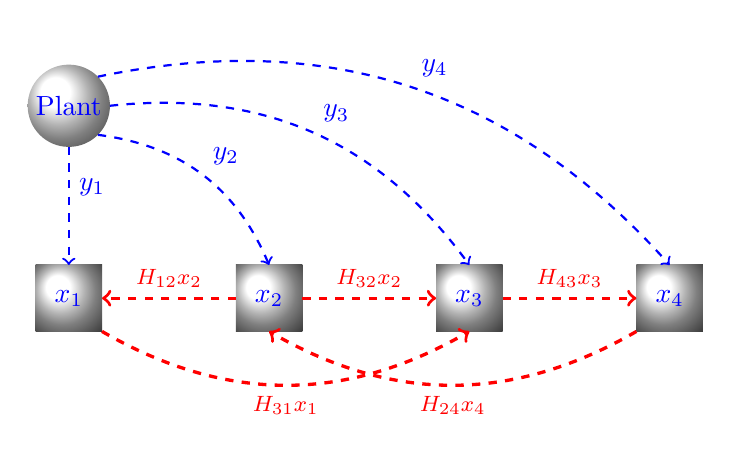
\begin{tikzpicture}[node distance=1.7cm]
  \tikzset{VertexStyle/.style = {shape          = circle,
                                 ball color     = white!20,
                                 text           = blue,
                                 inner sep      = 2pt,
                                 outer sep      = 0pt,
                                 minimum size   = 24 pt}}

     \node[VertexStyle,rectangle](A){ \math{x_{1}} };
     \node[VertexStyle,rectangle,right=of A](B){\math{x_{2}}};
     \node[VertexStyle,rectangle,right=of B](C){\math{x_{3}}};
     \node[VertexStyle,rectangle,right=of C](D){\math{x_{4}}};
     \node[VertexStyle,above=1.5cm of A](P){Plant};

     \draw[thick,->,dashed,blue](P.south) to node[above right]{ \math{y_{1}} } (A.north);
     \draw[thick,->,dashed,blue,bend left](P.south east) to node[above right]{ \math{y_{2}} } (B.north);
     \draw[thick,->,dashed,blue,bend left](P.east) to node[above right]{ \math{y_{3}} } (C.north);
     \draw[thick,->,dashed,blue,bend left](P.north east) to node[above right]{ \math{y_{4}} } (D.north);

     \draw[very thick,->,dashed,red](B.west) to node[above]{\footnotesize\math{H_{12}x_{2}}} (A.east);
     \draw[very thick,->,dashed,red](B.east) to node[above]{\footnotesize\math{H_{32}x_{2}}} (C.west);
     \draw[very thick,->,dashed,red](C.east) to node[above]{\footnotesize\math{H_{43}x_{3}}} (D.west);

     \draw[very thick,->,dashed,bend right,red](A.south east) to node[below]{\footnotesize\math{H_{31}x_{1}}} (C.south);
     \draw[very thick,->,dashed,bend left,red](D.south west) to node[below]{\footnotesize\math{H_{24}x_{4}}} (B.south);
\end{tikzpicture}
\end{center}

\textbf{Question (to reduce the communication burden):} The design communication gain matrix $H_{ij}$ is restricted, merely relating to output gain $C_{j}$ for $i\neq j\in\mathcal{N}_{i}$

\end{frame}
%%--------------------------------------------------------




%%========================================================
\section{Review of Paper: HTWS TAC-64(1)-2019}%

%%--------------------------------------------------------
\begin{frame}
\thispagestyle{empty}

\begin{center}
{\large\bf\color{blue}Paper: HTWS TAC-64(1)-2019 \\
{\footnotesize ``A Simple Approach to Distributed Observer Design for Linear Systems''} \\
{\footnotesize By W.~Han, H.~L.~Trentelman, Z.~Wang, and Y.~Shen}}
\end{center}
\end{frame}
%%--------------------------------------------------------



\subsection{\ding{228}~Introduction}%

%%--------------------------------------------------------
\begin{frame}{\color{blue} Plant and graph}

Consider LTI plant in state-space form
\begin{align*}
\dot{x}(t)&=A x(t) \\
y_{i}(t)&=C_{i}x(t),~~ x\in\R^{n},~~ y_{i}\in\R^{s_{i}},~~ i\in{\bf m}\triangleq \{1,2,\cdots,m\}
\end{align*}
Suppose that
\begin{equation*}
(C,A) ~~\text{with}~~ C=\begin{bmatrix} C_{1} \\ \vdots \\ C_{m} \\   \end{bmatrix}\in\R^{r} ~~\text{is observable}
\end{equation*}
For each $i\in{\bf m}$,
\begin{center}
$\mathcal{N}_{i}$ is the neighbors (without self-loops) of the $i$th observer
\end{center}
\end{frame}
%%--------------------------------------------------------






%%--------------------------------------------------------
\begin{frame}{\color{blue} Illustration}

\begin{center}
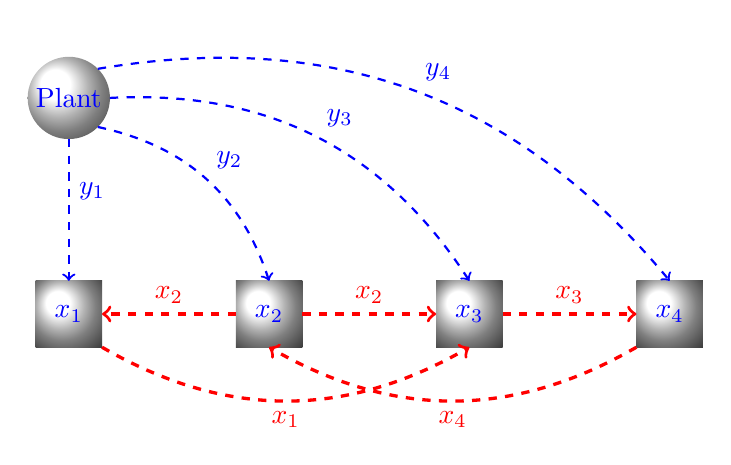
\begin{tikzpicture}[node distance=1.7cm]
  \tikzset{VertexStyle/.style = {shape          = circle,
                                 ball color     = white!20,
                                 text           = blue,
                                 inner sep      = 2pt,
                                 outer sep      = 0pt,
                                 minimum size   = 24 pt}}

     \node[VertexStyle,rectangle](A){ \math{x_{1}} };
     \node[VertexStyle,rectangle,right=of A](B){\math{x_{2}}};
     \node[VertexStyle,rectangle,right=of B](C){\math{x_{3}}};
     \node[VertexStyle,rectangle,right=of C](D){\math{x_{4}}};
     \node[VertexStyle,above=1.8cm of A](P){Plant};

     \draw[thick,->,dashed,blue](P.south) to node[above right]{ \math{y_{1}} } (A.north);
     \draw[thick,->,dashed,blue,bend left](P.south east) to node[above right]{ \math{y_{2}} } (B.north);
     \draw[thick,->,dashed,blue,bend left](P.east) to node[above right]{ \math{y_{3}} } (C.north);
     \draw[thick,->,dashed,blue,bend left](P.north east) to node[above right]{ \math{y_{4}} } (D.north);

     \draw[very thick,->,dashed,red](B.west) to node[above]{\math{x_{2}}} (A.east);
     \draw[very thick,->,dashed,red](B.east) to node[above]{\math{x_{2}}} (C.west);
     \draw[very thick,->,dashed,red](C.east) to node[above]{\math{x_{3}}} (D.west);

     \draw[very thick,->,dashed,bend right,red](A.south east) to node[below]{\math{x_{1}}} (C.south);
     \draw[very thick,->,dashed,bend left,red](D.south west) to node[below]{\math{x_{4}}} (B.south);
\end{tikzpicture}
\end{center}

\begin{align*}
m&=4,~~ {\bf m}\triangleq \{1,2,3,4\} \\
\mathcal{N}_{1}&=\{2\},~~ \mathcal{N}_{2}=\{4\},~~ \mathcal{N}_{3}=\{1,2\},~~ \mathcal{N}_{4}=\{3\}
\end{align*}

\end{frame}
%%--------------------------------------------------------




\subsection{\ding{228}~Main Theorem}%

%%--------------------------------------------------------
\begin{frame}{\color{blue} Distributed observer by HTWS 2019TAC}

Structure of the distributed \textbf{(identical)} observer by HTWS 2019TAC
\begin{align*}
\dot{x}_{i}(t)&=A x_{i} +L_{i}(y_{i}-C_{i}x_{i})+\gamma M_{i} \sum_{j\in\mathcal{N}_{i}} a_{ij}\big(x_{j}(t)-x_{i}(t) \big),~~ i\in{\bf m}
\end{align*}
It is hoped to achieve convergence of the estimation error
\begin{equation*}
\lim_{t\rightarrow\infty} |\epsilon_{i}(t)|=0,~~ \epsilon_{i}(t)=x_{i}(t)-x(t),~~ \forall i\in{\bf m}
\end{equation*}

\textbf{Main Theorem.} Assume
\begin{itemize}
  \item $(C,A)$ is (jointly) observable and
  \item $\mathcal{G}$ is a strongly connected directed graph.
\end{itemize}
Then there exists a distributed observer that achieves omniscience asymptotically.


\end{frame}
%%--------------------------------------------------------






\subsection{\ding{228}~Remark}%


%%--------------------------------------------------------
\begin{frame}{\color{blue} Remark on HTWS 2019TAC}

The distributed \textbf{(identical)} observer by HTWS 2019TAC
\begin{align*}
\dot{x}_{i}(t)&=A x_{i} +L_{i}(y_{i}-C_{i}x_{i})+\gamma M_{i} \sum_{j\in\mathcal{N}_{i}} a_{ij}\big(x_{j}(t)-x_{i}(t) \big),~~ i\in{\bf m}
\end{align*}
Assume
\begin{itemize}
  \item $(C,A)$ is (jointly) observable and
  \item $\mathcal{G}$ is a strongly connected directed graph.
\end{itemize}

{\color{red}\bf Remark.}
\begin{itemize}
  \item The plant matrix $A$ should be the \emph{a prior} or precisely known
  \item The communication signal at each edge is
\begin{equation*}
\gamma a_{ij} M_{i} x_{j}(t)
\end{equation*}
possibly burdensome!
\end{itemize}


\end{frame}
%%--------------------------------------------------------





%%========================================================
\section{Our Project}%

%%--------------------------------------------------------
\begin{frame}
\thispagestyle{empty}

\begin{center}
{\Large\bf\color{blue}Our Project/Plan \\
{\small  Distributed observers based on output interactions: \\ Necessary and sufficient conditions} }
\end{center}

Hope to achieve distributed estimation of
\begin{itemize}
  \item less communications
  \item arbitrary convergence rate
  \item easy to implement
\end{itemize}

\end{frame}
%%--------------------------------------------------------



\subsection{\ding{228}~Conjecture}%

%%--------------------------------------------------------
\begin{frame}{\color{blue} Plant and graph}

Consider LTI plant in state-space form
\begin{align*}
\dot{x}(t)&=A x(t) \\
y_{i}(t)&=C_{i}x(t),~~ x\in\R^{n},~~ y_{i}\in\R,~~ i\in{\bf m}\triangleq \{1,2,\cdots,m\}
\end{align*}
with \textbf{single outputs}. Suppose that
\begin{equation*}
(C,A) ~~\text{with}~~ C=\begin{bmatrix} C_{1} \\ \vdots \\ C_{m} \\   \end{bmatrix}\in\R^{m} ~~\text{is observable}
\end{equation*}
For each $i\in{\bf m}$,
\begin{center}
$\mathcal{N}_{i}$ is the neighbors \textbf{(without self-loops)} of the $i$th observer
\end{center}
\end{frame}
%%--------------------------------------------------------





%%--------------------------------------------------------
\begin{frame}{\color{blue} Assumption}
\begin{itemize}
  \item \textbf{Assumption}
\begin{itemize}
  \item [\bf A1] $A$ has no eigenvalue with negative real part, and
  \item [\bf A2] $\mathcal{G}$ is a directed graph such that, for each $i\in{\bf m}$,
\begin{equation*}
(\bar{C}_{i},A)  ~~\text{is observable}
\end{equation*}
(namely, locally jointly observable) where
\begin{align*}
\bar{C}_{i}=\begin{bmatrix} C_{i} \\ C_{j},j\in\mathcal{N}_{i} \\ \end{bmatrix} =\begin{bmatrix} C_{i} \\ C_{j_{1}} \\ \vdots \\ C_{j_{l_{i}}} \\ \end{bmatrix},~~ l_{i}=|\mathcal{N}_{i}| \\
j_{1}<\cdots<j_{l_{i}},~~ j_{k}\in\mathcal{N}_{i},~~ k=1,\cdots, l_{i}
\end{align*}
\end{itemize}

  \item \textbf{Remark} The above condition {\bf A2} is stronger than
\begin{center}
{\color{red}$(C,A)$ is (jointly) observable}
\end{center}
\end{itemize} 


\end{frame}
%%--------------------------------------------------------




%%--------------------------------------------------------
\begin{frame}{\color{blue} Structure of the distributed observers}

Consider the distributed observer design, taking the form
\begin{align*}
\Sigma_{obs}:~~ \dot{z}_{i}&=M_{i}z_{i}+ N_{i}\begin{bmatrix} y_{i} \\ \hat{y}_{j},j\in\mathcal{N}_{i} \\ \end{bmatrix} \\
\hat{x}_{i}&=\Gamma_{i}z_{i},~~ z_{i}\in\R^{n},~~ i\in{\bf m}
\end{align*}
or written by
\begin{align*}
\Sigma_{obs}:~~ \dot{z}_{i}&=M_{i}z_{i}+ N_{i}\begin{bmatrix} C_{i}x \\ C_{j}\hat{x}_{j},j\in\mathcal{N}_{i} \\ \end{bmatrix} \\
&=M_{i}z_{i} + N_{i}\begin{bmatrix} C_{i}x \\ C_{j}x,j\in\mathcal{N}_{i} \\ \end{bmatrix} + N_{i}\begin{bmatrix} 0 \\ C_{j}\hat{x}_{j}-C_{j}x,j\in\mathcal{N}_{i} \\ \end{bmatrix} \\
&=M_{i}z_{i}+ N_{i} \bar{C}_{i} x +N_{i}\begin{bmatrix} 0 \\ C_{j} \hat{x}_{j}-C_{j} x,j\in\mathcal{N}_{i} \\ \end{bmatrix} \\
\hat{x}_{i}&=\Gamma_{i}z_{i},~~ i\in{\bf m}
\end{align*}

\end{frame}
%%--------------------------------------------------------




%%--------------------------------------------------------
\begin{frame}{\color{blue} Necessary condition}


\begin{itemize}
  \item [C1] \textbf{(invariance)} For each $i\in{\bf m}$, there is a \textbf{non-singular matrix} $\Pi_{i}\in\R^{n\times n}$ such that
\begin{align*}
\Pi_{i}A&=M_{i}\Pi_{i}+ N_{i}\bar{C}_{i},~~ 0=I_{n}-\Gamma_{i}\Pi_{i},~~ \Gamma_{i}=\Pi_{i}^{-1},~~ i\in{\bf m}
\end{align*}
  \item [C2] \textbf{(convergence or stability)} Moreover, letting
\begin{equation*}
\epsilon_{i}=z_{i}-\Pi_{i}x,~~ \epsilon=\begin{bmatrix} \epsilon_{1}^{T} & \cdots & \epsilon_{m}^{T} \\ \end{bmatrix}^{T}
\end{equation*}
the error system
\begin{align*}
\dot{\epsilon}_{i}%&=M_{i}\epsilon_{i} +N_{i}\begin{bmatrix} 0 \\ C_{j} \Gamma_{j}z_{j}-C_{j} x,j\in\mathcal{N}_{i} \\ \end{bmatrix} \\
&=M_{i}\epsilon_{i} +N_{i}\begin{bmatrix} 0 \\ C_{j} \Gamma_{j}(\epsilon_{j}+\Pi_{j}x)-C_{j}x,j\in\mathcal{N}_{i} \\ \end{bmatrix} \\
&=M_{i}\epsilon_{i} +N_{i}\begin{bmatrix} 0 \\ C_{j} \Gamma_{j}\epsilon_{j},j\in\mathcal{N}_{i} \\ \end{bmatrix},~~ i\in{\bf m}
\end{align*}
or written in the compact form
\begin{align*}
\dot{\epsilon}&=M \epsilon
\end{align*}
should be asymptotically stable at $\epsilon=0$
\end{itemize}
\end{frame}
%%--------------------------------------------------------



%%--------------------------------------------------------
\begin{frame}{\color{blue}\bf Conjecture }

If
\begin{itemize}
  \item [\bf A1] $A$ has no eigenvalue with negative real part, and
  \item [\bf A2] $\mathcal{G}$ is a directed graph such that, for each $i\in{\bf m}$,
\begin{equation*}
(\bar{C}_{i},A)  ~~\text{is observable}
\end{equation*}
\end{itemize}
then, there are design parameters $\{M_{i},N_{i},\Gamma_{i}\}$ for $i\in{\bf m}$ satisfying the following conditions:
\begin{itemize}
  \item [C1] \textbf{(invariance)} There are matrices $\Pi_{i}$ for $i\in{\bf m}$ such that
\begin{align*}
\Pi_{i}A&=M_{i}\Pi_{i}+ N_{i}\bar{C}_{i},~~ 0=I_{n}-\Gamma_{i}\Pi_{i},~~ i\in{\bf m}
\end{align*}
  \item [C2] \textbf{(convergence or stability)} Moreover, the error system
\begin{align*}
\dot{\epsilon}&=M \epsilon
\end{align*}
is asymptotically stable at $\epsilon=0$
\end{itemize}

\end{frame}
%%--------------------------------------------------------




%%--------------------------------------------------------
\begin{frame}{\color{blue} Not true!}

The error system is
\begin{align*}
\dot{\epsilon}_{i}&=M_{i}\epsilon_{i} +N_{i}\begin{bmatrix} 0 \\ C_{j} \Gamma_{j}\epsilon_{j},j\in\mathcal{N}_{i} \\ \end{bmatrix},~~ i\in{\bf m}
\end{align*}
Without loss of generality, suppose the controllable pair $(M_{i},N_{i})$ is diagonal,
\begin{align*}
M_{i}=\begin{bmatrix} M_{i1} & 0 \\ 0 & M_{i2} \\ \end{bmatrix},~~ N_{i}=\begin{bmatrix} N_{i1} & 0 \\ 0 & N_{i2} \\ \end{bmatrix}
\end{align*}
with $M_{i}$ being Hurwitz. Also, let
\begin{align*}
\epsilon_{i}&=\begin{bmatrix} \epsilon_{i1} \\ \epsilon_{i2} \\ \end{bmatrix},~~
\begin{bmatrix} N_{i2}C_{j} \Gamma_{j}\epsilon_{j},j\in\mathcal{N}_{i} \\ \end{bmatrix}
=\begin{bmatrix} \bar{\Gamma}_{i1} &  &  \\ & \ddots &  \\  & & \bar{\Gamma}_{i,2m} \\ \end{bmatrix}\begin{bmatrix} \epsilon_{11} \\ \vdots \\ \epsilon_{m2} \\ \end{bmatrix}=:\bar{\Gamma}_{i}\epsilon
\end{align*}
with (because $j\neq i$)
\begin{equation*}
\bar{\Gamma}_{i,2i-1}=0,~~ \bar{\Gamma}_{i,2i}=0
\end{equation*}

\end{frame}
%%--------------------------------------------------------





%%--------------------------------------------------------
\begin{frame}{\color{blue} }

It gives
\begin{align*}
\dot{\epsilon}_{i1}&=M_{i1}\epsilon_{i1} \\
\dot{\epsilon}_{i2}&=M_{i2}\epsilon_{i2} + \bar{\Gamma}_{i}\epsilon,~~ i\in{\bf m}
\end{align*}
and
\begin{align*}
\dot{\epsilon}&=\left[\begin{array}{ll|ll|c|ll}
                  M_{11} & 0 &  0 & 0  & \cdots &  0  & 0 \\
                  0 & M_{12}  & \bar{\Gamma}_{13}  & \bar{\Gamma}_{14}  & \cdots &  \bar{\Gamma}_{1,2m-1}  & \bar{\Gamma}_{1,2m} \\ \hline
                  0 & 0 & M_{21} & 0 & \cdots &  0  & 0 \\
                  \bar{\Gamma}_{21}  & \bar{\Gamma}_{22}  & 0 & M_{12} & \cdots & \bar{\Gamma}_{2,2m-1}  & \bar{\Gamma}_{2,2m} \\ \hline
                  \vdots &   &  \vdots  &    & \ddots &  \vdots   & \\ \hline
                  0 & 0 &  0 & 0  & \cdots &  M_{m1}  & 0 \\
                  \bar{\Gamma}_{m1} & \bar{\Gamma}_{m2}  & \bar{\Gamma}_{m3}  & \bar{\Gamma}_{m4}  & \cdots & 0 & M_{m2} \\
                \end{array}\right]\epsilon=:\mathcal{M}\epsilon
\end{align*}

Is $\mathcal{M}$ Hurwitz? Or, any additional condition?
\end{frame}
%%--------------------------------------------------------





%%--------------------------------------------------------
\begin{frame}{\color{blue} }

\begin{columns}[onlytextwidth]
\column{0.5\textwidth}
Interconnection structure of
\begin{equation*}
\dot{\epsilon}=\mathcal{M}\epsilon
\end{equation*}

\column{0.5\textwidth}
\begin{center}
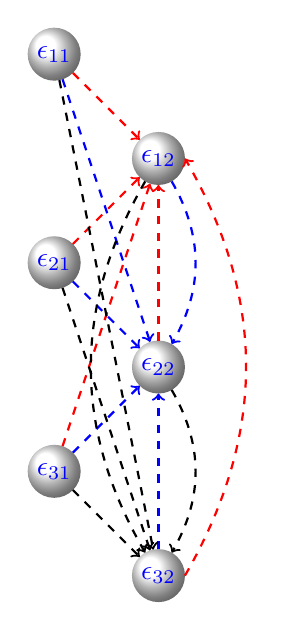
\begin{tikzpicture}[node distance=1.2cm]
  \tikzset{VertexStyle/.style = {shape          = circle,
                                 ball color     = white!20,
                                 text           = blue,
                                 inner sep      = 2pt,
                                 outer sep      = 0pt,
                                 minimum size   = 10 pt}}
     \node[VertexStyle](A1){ \math{\epsilon_{11}} };
     \node[VertexStyle,below right=of A1](A2){\math{\epsilon_{12}}};
     \node[VertexStyle,below left=of A2](B1){\math{\epsilon_{21}}};
     \node[VertexStyle,below right=of B1](B2){\math{\epsilon_{22}}};
     \node[VertexStyle,below left=of B2](C1){\math{\epsilon_{31}}};
     \node[VertexStyle,below right=of C1](C2){\math{\epsilon_{32}}};

     \draw[thick,->,dashed,red](A1) to (A2);
     \draw[thick,->,dashed,red](B1) to (A2);
     \draw[thick,->,dashed,red](B2) to (A2);
     \draw[thick,->,dashed,red](C1) to (A2);
     \draw[thick,->,dashed,red,bend right](C2.east) to (A2.east);

     \draw[thick,->,dashed,blue](B1) to (B2);
     \draw[thick,->,dashed,blue](A1) to (B2);
     \draw[thick,->,dashed,blue,bend left](A2) to (B2);
     \draw[thick,->,dashed,blue](C1) to (B2);
     \draw[thick,->,dashed,blue](C2) to (B2);

     \draw[thick,->,dashed,black](C1) to (C2);
     \draw[thick,->,dashed,black](A1) to (C2);
     \draw[thick,->,dashed,black,bend right](A2) to (C2);
     \draw[thick,->,dashed,black](B1) to (C2);
     \draw[thick,->,dashed,black,bend left](B2) to (C2);
\end{tikzpicture}
\end{center}
\end{columns}
\end{frame}
%%--------------------------------------------------------





%%--------------------------------------------------------
\begin{frame}{\color{blue} }

\begin{columns}[onlytextwidth]
\column{0.5\textwidth}
Interconnection structure of
\begin{equation*}
\dot{\epsilon}=\mathcal{M}\epsilon
\end{equation*}

Removing $\epsilon_{11}$ to $\epsilon_{m1}$ subsystems gives

\begin{align*}
\dot{\epsilon}'&=\left[\begin{array}{l|l|c|l}
                  M_{12}  & \bar{\Gamma}_{14}  & \cdots &  \bar{\Gamma}_{1,2m} \\ \hline
                  \bar{\Gamma}_{22}  & M_{12} & \cdots & \bar{\Gamma}_{2,2m} \\ \hline
                  \vdots  &    & \ddots &  \vdots \\ \hline
                  \bar{\Gamma}_{m2}  & \bar{\Gamma}_{m4}  & \cdots & M_{m2} \\
                \end{array}\right]\epsilon' \\
&=:\mathcal{M}'\epsilon'
\end{align*}

Note that if $\mathcal{M}'$ is Hurwitz, then $\mathcal{M}$ is so


\column{0.5\textwidth}
\begin{center}
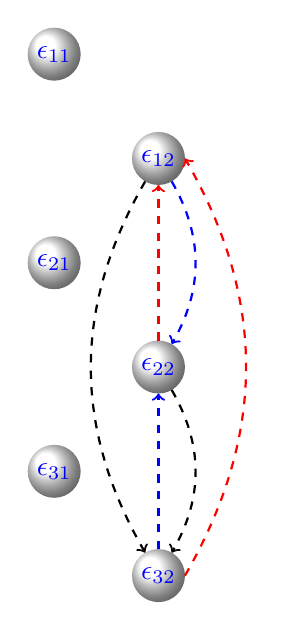
\begin{tikzpicture}[node distance=1.2cm]
  \tikzset{VertexStyle/.style = {shape          = circle,
                                 ball color     = white!20,
                                 text           = blue,
                                 inner sep      = 2pt,
                                 outer sep      = 0pt,
                                 minimum size   = 10 pt}}
     \node[VertexStyle](A1){ \math{\epsilon_{11}} };
     \node[VertexStyle,below right=of A1](A2){\math{\epsilon_{12}}};
     \node[VertexStyle,below left=of A2](B1){\math{\epsilon_{21}}};
     \node[VertexStyle,below right=of B1](B2){\math{\epsilon_{22}}};
     \node[VertexStyle,below left=of B2](C1){\math{\epsilon_{31}}};
     \node[VertexStyle,below right=of C1](C2){\math{\epsilon_{32}}};

     %\draw[thick,->,dashed,red](A1) to (A2);
     %\draw[thick,->,dashed,red](B1) to (A2);
     \draw[thick,->,dashed,red](B2) to (A2);
     %\draw[thick,->,dashed,red](C1) to (A2);
     \draw[thick,->,dashed,red,bend right](C2.east) to (A2.east);

     %\draw[thick,->,dashed,blue](B1) to (B2);
     %\draw[thick,->,dashed,blue](A1) to (B2);
     \draw[thick,->,dashed,blue,bend left](A2) to (B2);
     %\draw[thick,->,dashed,blue](C1) to (B2);
     \draw[thick,->,dashed,blue](C2) to (B2);

     %\draw[thick,->,dashed,green](C1) to (C2);
     %\draw[thick,->,dashed,green](A1) to (C2);
     \draw[thick,->,dashed,black,bend right](A2) to (C2);
     %\draw[thick,->,dashed,green](B1) to (C2);
     \draw[thick,->,dashed,black,bend left](B2) to (C2);
\end{tikzpicture}
\end{center}
\end{columns}
\end{frame}
%%--------------------------------------------------------



%%--------------------------------------------------------
\begin{frame}{\color{blue} Example}

\begin{itemize}
  \item Plant
\begin{align*}
& x\in\R^{4},~~ A=\begin{bmatrix} A_{1} & 0 \\ 0 & A_{2} \\ \end{bmatrix},~~ A_{i}=\begin{bmatrix} 0 & 1 \\ -\sigma_{i} & 0 \\ \end{bmatrix},~~ \sigma_{i}>0,~~ m=2
\end{align*}

  \item \textbf{Case-I}
\begin{equation*}
C_{1}=\begin{bmatrix} 1 & 0 & 1 & 0 \\ \end{bmatrix},~~ C_{2}=C_{1}
\end{equation*}
In this case
\begin{align*}
\Sigma_{obs}^{(1)}:~~ \dot{z}_{1}&=M_{1}z_{1}+ N_{1}\begin{bmatrix} y_{1} \\ \hat{y}_{2} \\ \end{bmatrix},~~ M_{1}\in\R^{4\times4},~~ N_{1}\in\R^{4\times2} \\
\Sigma_{obs}^{(2)}:~~ \dot{z}_{2}&=M_{2}z_{2}+ N_{2}\begin{bmatrix} y_{2} \\ \hat{y}_{1} \\ \end{bmatrix},~~ M_{2}\in\R^{4\times4},~~ N_{2}\in\R^{4\times2}
\end{align*}
\end{itemize}

\end{frame}
%%--------------------------------------------------------




%%--------------------------------------------------------
\begin{frame}{\color{blue} }

\begin{itemize}

  \item Observers
\begin{align*}
\Sigma_{obs}^{(1)}:~~ \dot{z}_{1}&=M_{1}z_{1}+ N_{1}\begin{bmatrix} C_{1}x \\ C_{2}\hat{x}_{2} \\ \end{bmatrix},~~ M_{1}\in\R^{4\times4},~~ N_{1}\in\R^{4\times2} \\
\Sigma_{obs}^{(2)}:~~ \dot{z}_{2}&=M_{2}z_{2}+ N_{2}\begin{bmatrix} C_{2}x \\ C_{1}\hat{x}_{1} \\ \end{bmatrix},~~ M_{2}\in\R^{4\times4},~~ N_{2}\in\R^{4\times2}
\end{align*}
Then, we write the error systems
\begin{align*}
\Sigma_{obs}^{(1)}:~~ \dot{z}_{1}&=M_{1}z_{1}+ N_{1}\bar{C}_{1}x + N_{1}\begin{bmatrix} 0 \\ C_{2}\hat{x}_{2}-C_{2}x \\ \end{bmatrix} \\
\dot{\epsilon}_{1}&=M_{1}\epsilon_{1}+ N_{1}\begin{bmatrix} 0 \\ C_{2}\epsilon_{2} \\ \end{bmatrix} \\
\Sigma_{obs}^{(2)}:~~ \dot{z}_{2}&=M_{2}z_{2}+ N_{2}\bar{C}_{2}x + N_{2}\begin{bmatrix} 0 \\ C_{1}\hat{x}_{1}-C_{1}x \\ \end{bmatrix} \\
\dot{\epsilon}_{2}&=M_{2}\epsilon_{2}+ N_{2}\begin{bmatrix} 0 \\ C_{1}\epsilon_{1} \\ \end{bmatrix}
\end{align*}

\end{itemize}

\end{frame}
%%--------------------------------------------------------




%%--------------------------------------------------------
\begin{frame}{\color{blue} }

\begin{itemize}

  \item Now, consider the error systems
\begin{align*}
\dot{\epsilon}_{1}&=M_{1}\epsilon_{1}+ N_{1}\begin{bmatrix} 0 \\ C_{2}\epsilon_{2} \\ \end{bmatrix} \\
\dot{\epsilon}_{2}&=M_{2}\epsilon_{1}+ N_{2}\begin{bmatrix} 0 \\ C_{1}\epsilon_{1} \\ \end{bmatrix}
\end{align*}

  \item {\bf\color{red}Caution}  $(M_{i},N_{i})$ for $i=1,2$ are not diagonalizable!

\end{itemize}

\end{frame}
%%--------------------------------------------------------



%%--------------------------------------------------------
\begin{frame}{\color{blue} Scenario I}


\begin{columns}[onlytextwidth]
\column{0.5\textwidth}
\textbf{Assumption}
\begin{itemize}
  \item [\bf A1] $A$ has no eigenvalue with negative real part 
  \item [\bf A2] $\mathcal{G}$ is a directed graph such that, for each $i\in{\bf m}$,
\begin{equation*}
(\bar{C}_{i},A) ~~\text{is observable}
\end{equation*}
where
\begin{align*}
\bar{C}_{i}=\begin{bmatrix} C_{i} \\ C_{j},j\in\mathcal{N}_{i} \\ \end{bmatrix}
\end{align*}
(locally jointly observable)
\end{itemize}

\column{0.5\textwidth}
\begin{center}
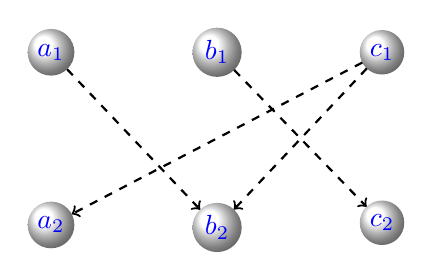
\begin{tikzpicture}[node distance=1.6cm]
  \tikzset{VertexStyle/.style = {shape          = circle,
                                 ball color     = white!20,
                                 text           = blue,
                                 inner sep      = 2pt,
                                 outer sep      = 0pt,
                                 minimum size   = 10 pt}}
     \node[VertexStyle](A1){ \math{a_{1}} };
     \node[VertexStyle,below=of A1](A2){\math{a_{2}}};
     \node[VertexStyle,right=1.5cm of A1](B1){\math{b_{1}}};
     \node[VertexStyle,below=of B1](B2){\math{b_{2}}};
     \node[VertexStyle,right=1.5cm of B1](C1){\math{c_{1}}};
     \node[VertexStyle,below=of C1](C2){\math{c_{2}}};

     \draw[thick,->,dashed](A1) to (B2);
     \draw[thick,->,dashed](B1) to (C2);
     \draw[thick,->,dashed](C1) to (A2);
     \draw[thick,->,dashed](C1) to (B2);
\end{tikzpicture}
\end{center}

\begin{align*}
\Sigma_{obs}:~~ \dot{z}_{i}&=M_{i}z_{i}+ N_{i}\begin{bmatrix} y_{i} \\ \hat{y}_{j},j\in\mathcal{N}_{i} \\ \end{bmatrix} \\
\hat{x}_{i}&=\Gamma_{i}z_{i},~~ z_{i}\in\R^{n},~~ i\in{\bf m}
\end{align*}
\end{columns} 

\end{frame}
%%--------------------------------------------------------





%%--------------------------------------------------------
\begin{frame}{\color{blue} Scenario II}


\begin{columns}[onlytextwidth]
\column{0.5\textwidth}
\textbf{Assumption}
\begin{itemize}
  \item [\bf A1] $A$ has no eigenvalue with negative real part
  \item [\bf A2] $(C,A)$ is jointly observable  
\end{itemize}

\vskip 1cm

The communication graph is
\begin{center}
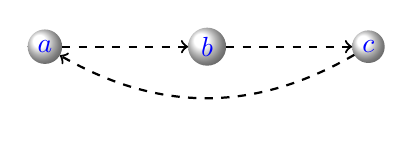
\begin{tikzpicture}[node distance=1.6cm]
  \tikzset{VertexStyle/.style = {shape          = circle,
                                 ball color     = white!20,
                                 text           = blue,
                                 inner sep      = 2pt,
                                 outer sep      = 0pt,
                                 minimum size   = 10 pt}}
     \node[VertexStyle](A){ \math{a} };
     \node[VertexStyle,right=of A](B){\math{b}};
     \node[VertexStyle,right=of B](C){\math{c}};

     \draw[thick,->,dashed](A) to (B);
     \draw[thick,->,dashed](B) to (C);
     \draw[thick,->,dashed,bend left](C) to (A);
\end{tikzpicture}
\end{center}


\column{0.5\textwidth}
\begin{center}
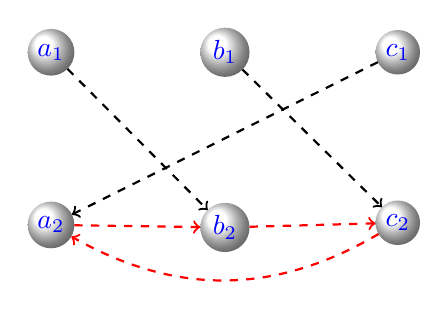
\begin{tikzpicture}[node distance=1.6cm]
  \tikzset{VertexStyle/.style = {shape          = circle,
                                 ball color     = white!20,
                                 text           = blue,
                                 inner sep      = 2pt,
                                 outer sep      = 0pt,
                                 minimum size   = 10 pt}}
     \node[VertexStyle](A1){ \math{a_{1}} };
     \node[VertexStyle,below=of A1](A2){\math{a_{2}}};
     \node[VertexStyle,right=of A1](B1){\math{b_{1}}};
     \node[VertexStyle,below=of B1](B2){\math{b_{2}}};
     \node[VertexStyle,right=of B1](C1){\math{c_{1}}};
     \node[VertexStyle,below=of C1](C2){\math{c_{2}}};

     \draw[thick,->,dashed](A1) to (B2);
     \draw[thick,->,dashed](B1) to (C2);
     \draw[thick,->,dashed](C1) to (A2); 
     \draw[thick,->,dashed,red,bend left](C2) to (A2); 
     \draw[thick,->,dashed,red](B2) to (C2); 
     \draw[thick,->,dashed,red](A2) to (B2); 
\end{tikzpicture}
\end{center} 
 
\end{columns}

\end{frame}
%%--------------------------------------------------------















%%--------------------------------------------------------
\begin{frame}{\color{blue} Modified distributed observers}

Consider LTI plant in state-space form
\begin{align*}
\dot{x}&=A x,~~ y_{i}=C_{i}x,~~ x\in\R^{n},~~ y_{i}\in\R,~~ i\in{\bf m}
\end{align*}

Consider a modified distributed observer
\begin{align*}
\Sigma_{obs}:~~ \dot{z}_{i}&=M_{i}z_{i}+ N_{i}\begin{bmatrix} y_{i} \\ \hat{y}_{j},j\in\mathcal{N}_{i} \\ \end{bmatrix}
{\color{red}+\gamma H_{i}\begin{bmatrix} \hat{y}_{j}-\hat{y}_{i}, j\in\mathcal{N}_{i} \\ \end{bmatrix}} \\
\hat{x}_{i}&=\Gamma_{i}z_{i},~~ i\in{\bf m}
\end{align*}
with
\begin{equation*}
\hat{y}_{i}=C_{i}\hat{x}_{i}
\end{equation*}
The error system is
\begin{align*}
\dot{\epsilon}_{i}&=M_{i}\epsilon_{i} +N_{i}\begin{bmatrix} 0 \\ C_{j} \Gamma_{j}\epsilon_{j},j\in\mathcal{N}_{i} \\ \end{bmatrix} +...
\end{align*}

\end{frame}
%%--------------------------------------------------------





%%--------------------------------------------------------
\begin{frame}{\color{blue} }


\end{frame}
%%--------------------------------------------------------


%%--------------------------------------------------------
\begin{frame}{\color{blue} }


\end{frame}
%%--------------------------------------------------------


%%--------------------------------------------------------
\begin{frame}{\color{blue} }


\end{frame}
%%--------------------------------------------------------










\end{document}



%%--------------------------------------------------------
\begin{frame}{\color{blue}}


\end{frame}
%%--------------------------------------------------------



\begin{columns}[onlytextwidth]
\column{0.5\textwidth}


\column{0.5\textwidth}

\end{columns}


\begin{block}{Default}
Block content.
\end{block}

\begin{alertblock}{Alert}
Block content.
\end{alertblock}

\begin{exampleblock}{Example}
Block content.
\end{exampleblock}


\begin{table}
\caption{Largest cities in the world (source: Wikipedia)}
\begin{tabular}{lr}
\toprule
City & Population\\
\midrule
Mexico City & 20,116,842\\
Shanghai & 19,210,000\\
Peking & 15,796,450\\
Istanbul & 14,160,467\\
\bottomrule
\end{tabular}
\end{table}
